\documentclass[10pt,a4paper]{article}
\usepackage[a4paper, top=2.0cm, bottom=2.2cm, left=2.2cm, right=2.2cm, headsep=0.6cm]{geometry}
\usepackage{fontspec}
\setmainfont{texgyretermes}[Extension=.otf, UprightFont=*-regular, BoldFont=*-bold, ItalicFont=*-italic, BoldItalicFont=*-bolditalic]
\setsansfont{texgyreheros}[Extension=.otf, UprightFont=*-regular, BoldFont=*-bold, ItalicFont=*-italic, BoldItalicFont=*-bolditalic]
\usepackage{babel}
\babelprovide[import, main]{polish}
\usepackage{microtype}
\usepackage{array, booktabs, longtable, tabularx}
\usepackage[table]{xcolor}
\usepackage{graphicx}
\usepackage{enumitem}
\usepackage{parskip}
\usepackage{fancyhdr}
\usepackage{titlesec}
\usepackage[hidelinks]{hyperref}
\emergencystretch=3em
\setlist{itemsep=2pt, topsep=3pt, leftmargin=1.4em}
\definecolor{L1}{HTML}{2A78D6}\definecolor{L2}{HTML}{EB6834}\definecolor{L3}{HTML}{1BAF7A}
\definecolor{L4}{HTML}{EDA100}\definecolor{L7}{HTML}{E87BA4}\definecolor{muted}{HTML}{767A84}
\definecolor{bad}{HTML}{C23030}\definecolor{good}{HTML}{0A8A0A}
\newcommand{\linedot}[1]{\textcolor{#1}{\rule[0.1ex]{0.9ex}{0.9ex}}\,}
\newcommand{\mut}[1]{\textcolor{muted}{#1}}
\titleformat{\section}{\sffamily\large\bfseries}{\thesection.}{0.5em}{}
\titleformat{\subsection}{\sffamily\normalsize\bfseries}{\thesubsection.}{0.5em}{}
\titlespacing*{\section}{0pt}{1.2em}{0.4em}
\titlespacing*{\subsection}{0pt}{0.9em}{0.3em}
\setlength{\LTpre}{4pt}\setlength{\LTpost}{4pt}
\pagestyle{fancy}\fancyhf{}
\renewcommand{\headrulewidth}{0.3pt}
\fancyhead[L]{\sffamily\footnotesize 14-200.pl/@yasiu/2026-09-30-raport-zkm}
\fancyhead[R]{\sffamily\footnotesize Przesiadki Iława Główna}
\fancyfoot[C]{\sffamily\footnotesize \thepage}
\begin{document}
{\sffamily\footnotesize\bfseries\MakeUppercase{Raport ZKM Iława · analiza rozkładów}}\par\smallskip
{\sffamily\LARGE\bfseries Przesiadki Iława Główna}\par\medskip
{\large Czy autobusy ZKM odjeżdżają spod dworca akurat wtedy, gdy przyjeżdżają pociągi?}\par\medskip
{\small\mut{Dworzec Iława Główna: 107 pociągów w dzień roboczy. Przystanek Dworcowa: linie ZKM 1, 2, 3, 4, 7, 106 odjazdów w dzień roboczy. Stan na 30.09.2026.}}\par\bigskip
\section*{Odpowiedź}
W dzień roboczy teza się nie potwierdza dla całej sieci. W dniu testowym (28.09.2026, rzeczywiste godziny pociągów) autobus odjeżdża w chwili przyjazdu pociągu przy \textbf{55\,\%} pociągów. Rozkład losowy daje \textbf{47\,\%} (90\,\% wyników losowych: 38\,\%--56\,\%). Wynik jest blisko górnej granicy losowości, ale mieści się w niej. Wrażenie „uciekającego autobusu” jest prawdziwe, ale wynika głównie z liczby kursów i skupień pociągów, a nie z ułożenia rozkładu. Rozkłady nie są ze sobą skoordynowane: według rozkładu planowego dobrych przesiadek (czekanie do 5 min) jest mniej więcej tyle, ile przy rozkładzie losowym. Wyjątkiem jest \textbf{linia 1} w dni robocze: autobus „ucieka” częściej niż losowo (24\,\% wobec 16\,\%). Chodzi głównie o 4 odjazdy po 17:00, po których następny kurs jest za 54--98 min. Sobota (26.09.2026, rzeczywiste godziny pociągów): autobus „ucieka” częściej niż przy 95\,\% rozkładów losowych (35\,\% wobec 27\,\%), więc tego dnia teza się potwierdza.

{\small
\begin{center}\begin{tabular}{@{}p{9.2cm} r p{4.2cm}@{}}\toprule
Wskaźnik & Wartość & Dla porównania \\ \midrule
Pociągi, którym autobus „ucieka” (dzień roboczy 28.09.2026) & 55\,\% & losowo 47\,\%; 86 przyjazdów \\
To samo dla linii 1 (dzień roboczy) & 24\,\% & losowo 16\,\%; wyżej niż w 97\,\% rozkładów losowych \\
Mediana opóźnienia pociągów PKP Intercity w Iławie & 3 min & POLREGIO: 0 min \\
Ciasne przesiadki z IC na daną linię (czekanie do 9 min), które się udają & 47\,\% & POLREGIO: 88\,\% \\
\bottomrule\end{tabular}\end{center}}
\section{Dni testowe: rozkład planowy i rzeczywiste godziny pociągów}
Rozkład ZKM jest ten sam każdego dnia danego typu, ale pociągi się spóźniają. Dlatego wyniki sprawdzono na minionych dniach, dla których są rzeczywiste godziny prawie wszystkich pociągów na stacji Iława Główna (monitor API PKP PLK). Dla każdego typu dnia dniem testowym jest dzień z największą liczbą pociągów spóźnionych ponad 5 min. Tabela podaje udział pociągów z dobrą przesiadką na dowolną linię dla okien czekania 5 min i 10 min: według planu / w rzeczywistości.

W dniu roboczym 28.09.2026 średnie opóźnienie przyjazdu wynosiło 12,0 min, a 24 z 93 pociągów przyjechało ponad 5 min po czasie. Przy oknie 5 min dobrą przesiadkę z pociągu na autobus miało 45\,\% pociągów według planu i 44\,\% w rzeczywistości; przy oknie 10 min: 67\,\% i 60\,\%.

{\footnotesize
\begin{center}\begin{tabular}{@{}l r r r r r r r@{}}\toprule
Dzień & Dane & Opóźn. śr./75\,\% & $>$5 min & P$\to$A 5 min & A$\to$P 5 min & P$\to$A 10 min & A$\to$P 10 min \\ \midrule
\textbf{26.09 sob.} & 89/92 & 2,8/3 min & 13 & 25\,\%/23\,\% & 26\,\%/27\,\% & 46\,\%/46\,\% & 40\,\%/47\,\% \\
\textbf{27.09 niedz.} & 91/91 & 21,7/7 min & 25 & 18\,\%/15\,\% & 15\,\%/16\,\% & 32\,\%/32\,\% & 28\,\%/28\,\% \\
\textbf{28.09 rob.} & 93/93 & 12,0/6 min & 24 & 45\,\%/44\,\% & 42\,\%/49\,\% & 67\,\%/60\,\% & 65\,\%/71\,\% \\
\bottomrule\end{tabular}\end{center}}
\mut{\footnotesize Pogrubienie: dzień testowy (rob.: dzień roboczy, sob.: sobota, niedz.: niedziela). P$\to$A: z pociągu na autobus, A$\to$P: z autobusu do pociągu, wartości: plan/rzeczywistość. Godziny autobusów są planowe, bo brak danych o faktycznych odjazdach. Spóźniony odjazd pociągu wydłuża czekanie na peronie, ale daje też czas autobusom, które według planu przyjeżdżają za późno.}
\section{Test tezy: rozkład rzeczywisty na tle losowego}
Dla każdego pociągu sprawdzono, czy autobus odjeżdża w chwili, gdy podróżni jeszcze idą z peronu na przystanek: od 2 min przed przyjazdem do 4 min po przyjeździe. Ten sam wskaźnik policzono 3000 razy dla rozkładu, w którym każdą linię przesunięto o losowy czas od $-30$ do $+30$ min. Szary pas to zakres 90\,\% wyników losowych, pionowa kreska to średnia losowa. Znacznik poza pasem oznacza wynik lepszy (zielony, trójkąt w stronę lepszego wyniku) albo gorszy (czerwony) niż losowo. Test używa rzeczywistych godzin pociągów z dnia testowego danego typu.

\par\medskip\noindent\begin{minipage}{\textwidth}\centering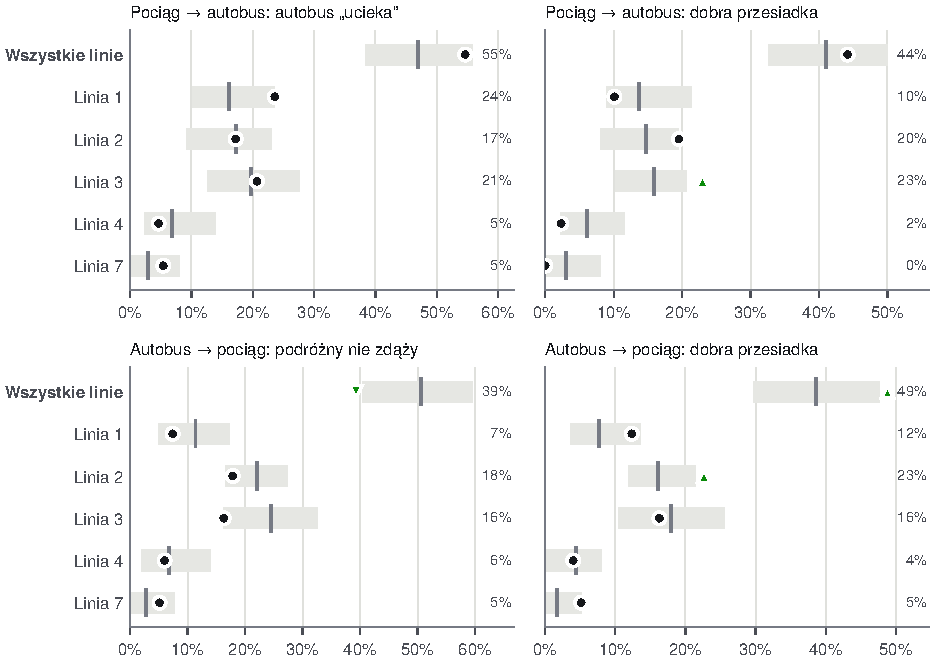
\includegraphics[width=\textwidth]{fig/przesiadki-test.pdf}\par\smallskip
{\small\mut{Rys. 1. Dzień roboczy 28.09.2026, rzeczywiste godziny pociągów. Test obejmuje pociągi w godzinach kursowania danej linii.}}\end{minipage}\par\medskip
Wszystkie linie razem, dzień testowy każdego typu (w nawiasie średnia losowa):
{\small
\begin{center}\begin{tabular}{@{}l r r r r@{}}\toprule
Typ dnia & Pociąg → autobus: ucieka & dobra & Autobus → pociąg: nie zdąży & dobra \\ \midrule
Dzień roboczy & 55\,\% \mut{(47\,\%)} & 44\,\% \mut{(41\,\%)} & 39\,\% \mut{(51\,\%)} & 49\,\% \mut{(39\,\%)} \\
Sobota & 35\,\% \mut{(27\,\%)} & 23\,\% \mut{(23\,\%)} & 21\,\% \mut{(28\,\%)} & 27\,\% \mut{(21\,\%)} \\
Niedziela i święta & 21\,\% \mut{(20\,\%)} & 15\,\% \mut{(17\,\%)} & 12\,\% \mut{(19\,\%)} & 16\,\% \mut{(14\,\%)} \\
\bottomrule\end{tabular}\end{center}}
\section{Kiedy odjeżdża autobus względem przyjazdu pociągu}
Każda para „pociąg -- autobus” w odstępie od $-20$ do $+30$ min, w przedziałach 2-minutowych. Gdyby autobusy uciekały pociągom, słupki w czerwonym polu byłyby wyraźnie wyższe od linii poziomu losowego. Gdyby rozkłady były skoordynowane, wyższe byłyby słupki w zielonym polu.
\par\medskip\noindent\begin{minipage}{\textwidth}\centering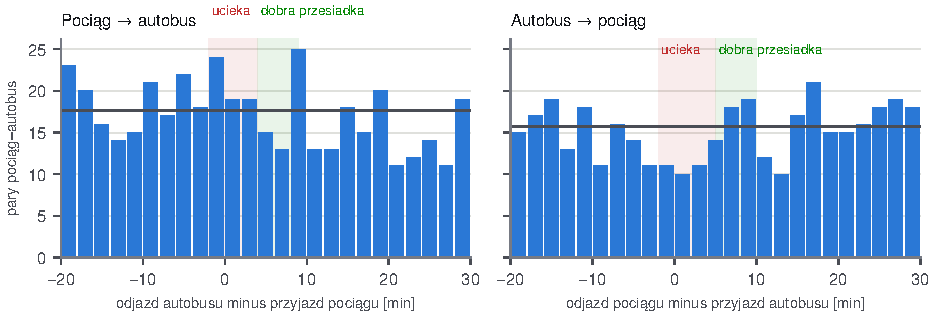
\includegraphics[width=\textwidth]{fig/przesiadki-odstepy.pdf}\par\smallskip
{\small\mut{Rys. 2. Dzień roboczy 28.09.2026, rzeczywiste godziny pociągów. Pozioma linia: poziom losowy.}}\end{minipage}\par\medskip
\section{Jeden dzień: przyjazdy pociągów i odjazdy autobusów}
Pionowe kreski to przyjazdy pociągów (długie: IC, EIP, EIC, TLK; krótkie: POLREGIO). Kropki to odjazdy autobusów spod dworca. Czerwona linia łączy pociąg z autobusem, który odjeżdża, zanim podróżni dojdą na przystanek.
\par\medskip\noindent\begin{minipage}{\textwidth}\centering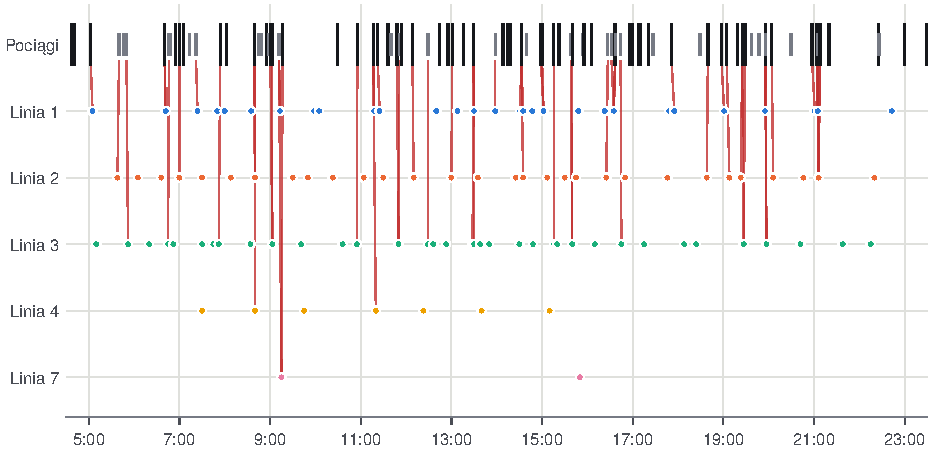
\includegraphics[width=\textwidth]{fig/przesiadki-dzien.pdf}\par\smallskip
{\small\mut{Rys. 3. Dzień roboczy 28.09.2026, rzeczywiste godziny pociągów.}}\end{minipage}\par\medskip
\section{Odjazdy, które „uciekają” pociągom}
Kursy, które w dniu testowym odjeżdżają w chwili przyjazdu co najmniej jednego pociągu, a następny kurs tej samej linii jest dopiero po 30 min lub później. Które z nich usuwa proponowana korekta, a które wymagają zmiany obiegu, pokazuje raport „Korekty rozkładu ZKM Iława”.
{\footnotesize
\begin{longtable}{@{}l l l p{4.1cm} l r@{}}\toprule
Dzień & Odjazd & Linia & Pociągi w tej chwili & Następny & Czekanie \\ \midrule\endhead
\bottomrule\endfoot
dzień roboczy & 05:05 & \linedot{L1}1 $\to$ Długa & 05:02 IC 5118 & 06:41 & 96 min \\
dzień roboczy & 06:42 & \linedot{L1}1 $\to$ Długa & 06:40 IC 5708 & 07:24 & 42 min \\
dzień roboczy & 07:00 & \linedot{L2}2 $\to$ Iława ul. Lipowy Dwór (ogrody) & 07:00 TLK 53104 & 07:30 & 30 min \\
dzień roboczy & 07:52 & \linedot{L3}3 $\to$ Nowa Wieś & 07:54 IC 1521 & 08:34 & 42 min \\
dzień roboczy & 08:40 & \linedot{L2}2 $\to$ Iława ul. Lipowy Dwór (ogrody) & 08:39 IC 1618 & 09:30 & 50 min \\
dzień roboczy & 08:40 & \linedot{L4}4 $\to$ Piaskowa & 08:39 IC 1618 & 09:45 & 65 min \\
dzień roboczy & 09:03 & \linedot{L3}3 $\to$ Nowa Wieś & 09:00 EIP 1503; 09:02 IC 5116 & 09:41 & 38 min \\
dzień roboczy & 09:13 & \linedot{L1}1 $\to$ Piaskowa & 09:12 R 90730 & 09:58 & 45 min \\
dzień roboczy & 09:15 & \linedot{L7}7 $\to$ Nowa Wieś (pętla, przejazd przez Dworcową) & 09:12 R 90730; 09:16 IC 7503 & 15:50 & 395 min \\
dzień roboczy & 10:55 & \linedot{L3}3 $\to$ Nowa Wieś & 10:55 EIP 5402 & 11:50 & 55 min \\
dzień roboczy & 11:20 & \linedot{L4}4 $\to$ Piaskowa & 11:16 IC 6115 & 12:23 & 63 min \\
dzień roboczy & 11:25 & \linedot{L1}1 $\to$ Długa & 11:22 EIP 4509 & 12:38 & 73 min \\
dzień roboczy & 11:50 & \linedot{L3}3 $\to$ Nowa Wieś & 11:48 IC 1511; 11:51 R 90654 & 12:29 & 39 min \\
dzień roboczy & 12:10 & \linedot{L2}2 $\to$ Iława ul. Lipowy Dwór (ogrody) & 12:08 EIP 3509 & 13:00 & 50 min \\
dzień roboczy & 13:00 & \linedot{L2}2 $\to$ Iława ul. Lipowy Dwór (ogrody) & 13:01 IC 5114 & 13:35 & 35 min \\
dzień roboczy & 13:58 & \linedot{L1}1 $\to$ Piaskowa & 13:58 R 90200 & 14:31 & 33 min \\
dzień roboczy & 14:35 & \linedot{L2}2 $\to$ Iława ul. Lipowy Dwór (ogrody) & 14:32 IC 5714 & 15:07 & 32 min \\
dzień roboczy & 15:02 & \linedot{L1}1 $\to$ Długa & 14:58 EIP 5304; 15:00 IC 1815 & 15:48 & 46 min \\
dzień roboczy & 15:40 & \linedot{L3}3 $\to$ Nowa Wieś & 15:38 R 90244; 15:40 IC 1515 & 16:10 & 30 min \\
dzień roboczy & 16:35 & \linedot{L1}1 $\to$ Długa & 16:32 R 90625; 16:36 IC 1614; 16:37 R 90225 & 17:48 & 73 min \\
dzień roboczy & 16:45 & \linedot{L3}3 $\to$ Nowa Wieś & 16:44 R 90656 & 17:15 & 30 min \\
dzień roboczy & 17:55 & \linedot{L1}1 $\to$ Długa & 17:51 EIP 5406 & 19:01 & 66 min \\
dzień roboczy & 18:38 & \linedot{L2}2 $\to$ Iława ul. Lipowy Dwór (ogrody) & 18:39 IC 5702 & 19:08 & 30 min \\
dzień roboczy & 19:01 & \linedot{L1}1 $\to$ Piaskowa & 18:57 IC 1517 & 19:55 & 54 min \\
dzień roboczy & 19:23 & \linedot{L2}2 $\to$ Iława ul. Lipowy Dwór (ogrody) & 19:25 IC 8114 & 20:06 & 43 min \\
dzień roboczy & 19:27 & \linedot{L3}3 $\to$ Nowa Wieś & 19:25 IC 8114; 19:28 IC 6119 & 19:57 & 30 min \\
dzień roboczy & 19:55 & \linedot{L1}1 $\to$ Długa & 19:55 EIP 5102; 19:56 R 90227 & 21:01 & 66 min \\
dzień roboczy & 19:57 & \linedot{L3}3 $\to$ Nowa Wieś & 19:55 EIP 5102; 19:56 R 90227 & 20:42 & 45 min \\
dzień roboczy & 20:06 & \linedot{L2}2 $\to$ Iława ul. Lipowy Dwór (ogrody) & 20:04 IC 5320 & 20:46 & 40 min \\
dzień roboczy & 21:05 & \linedot{L1}1 $\to$ Długa & 21:04 TLK 35105; 21:05 R 90113 & 22:43 & 98 min \\
dzień roboczy & 21:06 & \linedot{L2}2 $\to$ Iława ul. Lipowy Dwór (ogrody) & 21:04 TLK 35105; 21:05 R 90113; 21:07 EIP 3503; 21:08 TLK 53170 & 22:20 & 74 min \\
sobota & 05:42 & \linedot{L2}2 $\to$ Iława ul. Lipowy Dwór (ogrody) & 05:39 R 90621; 05:44 R 90205 & 06:15 & 33 min \\
sobota & 06:50 & \linedot{L1}1 $\to$ Długa & 06:47 R 90101; 06:50 R 90623 & 07:58 & 68 min \\
sobota & 07:04 & \linedot{L3}3 $\to$ Nowa Wieś & 07:03 TLK 35171; 07:06 TLK 53104 & 07:36 & 32 min \\
sobota & 07:54 & \linedot{L3}3 $\to$ Nowa Wieś & 07:55 IC 1521 & 08:26 & 32 min \\
sobota & 09:00 & \linedot{L3}3 $\to$ Nowa Wieś & 08:57 IC 1857; 09:00 IC 5116 & 09:45 & 45 min \\
sobota & 09:33 & \linedot{L1}1 $\to$ Piaskowa & 09:34 EIC 1541 & 10:05 & 32 min \\
sobota & 10:30 & \linedot{L1}1 $\to$ Piaskowa & 10:29 IC 5710 & 11:38 & 68 min \\
sobota & 11:10 & \linedot{L2}2 $\to$ Iława ul. Lipowy Dwór (ogrody) & 11:07 EIP 4509 & 12:01 & 51 min \\
sobota & 11:52 & \linedot{L3}3 $\to$ Nowa Wieś & 11:49 R 90654; 11:52 EIP 5302 & 12:35 & 43 min \\
sobota & 13:01 & \linedot{L2}2 $\to$ Iława ul. Lipowy Dwór (ogrody) & 12:59 EIP 5352; 13:00 IC 1815 & 14:11 & 70 min \\
sobota & 13:20 & \linedot{L1}1 $\to$ Długa & 13:16 IC 7515 & 14:53 & 93 min \\
sobota & 14:05 & \linedot{L3}3 $\to$ Nowa Wieś & 14:02 EIP 3507 & 14:35 & 30 min \\
sobota & 14:35 & \linedot{L3}3 $\to$ Nowa Wieś & 14:33 IC 5714 & 15:33 & 58 min \\
sobota & 15:00 & \linedot{L1}1 $\to$ Długa & 14:57 IC 1515 & 16:28 & 88 min \\
sobota & 15:10 & \linedot{L2}2 $\to$ Iława ul. Lipowy Dwór (ogrody) & 15:08 EIP 5304; 15:10 IC 8114 & 16:37 & 87 min \\
sobota & 16:37 & \linedot{L2}2 $\to$ Iława ul. Lipowy Dwór (ogrody) & 16:34 R 90625; 16:35 IC 1614 & 18:10 & 93 min \\
sobota & 21:06 & \linedot{L3}3 $\to$ Nowa Wieś & 21:03 R 90113; 21:05 EIP 3503; 21:07 EIC 5100 & brak & -- \\
niedziela & 07:07 & \linedot{L2}2 $\to$ Iława ul. Lipowy Dwór (ogrody) & 07:04 TLK 53104 & 09:00 & 113 min \\
niedziela & 09:00 & \linedot{L2}2 $\to$ Iława ul. Lipowy Dwór (ogrody) & 08:57 EIP 5400 & 10:51 & 111 min \\
niedziela & 09:16 & \linedot{L3}3 $\to$ Nowa Wieś & 09:13 IC 1553; 09:17 IC 7503 & 10:00 & 44 min \\
niedziela & 09:35 & \linedot{L1}1 $\to$ Długa & 09:33 EIC 1541 & 10:48 & 73 min \\
niedziela & 10:58 & \linedot{L1}1 $\to$ Długa & 10:57 EIP 5402 & 12:13 & 75 min \\
niedziela & 11:00 & \linedot{L3}3 $\to$ Nowa Wieś & 10:57 EIP 5402 & 11:46 & 46 min \\
niedziela & 11:46 & \linedot{L3}3 $\to$ Nowa Wieś & 11:48 R 90654 & 12:20 & 34 min \\
niedziela & 12:47 & \linedot{L1}1 $\to$ Długa & 12:43 IC 1706 & 14:08 & 81 min \\
niedziela & 14:38 & \linedot{L2}2 $\to$ Iława ul. Lipowy Dwór (ogrody) & 14:34 IC 5714; 14:38 R 55205 & 16:32 & 114 min \\
niedziela & 15:40 & \linedot{L1}1 $\to$ Długa & 15:38 R 90244 & 16:58 & 78 min \\
niedziela & 16:32 & \linedot{L2}2 $\to$ Iława ul. Lipowy Dwór (ogrody) & 16:34 R 90625 & 18:10 & 98 min \\
niedziela & 16:58 & \linedot{L1}1 $\to$ Piaskowa & 16:59 IC 5112 & brak & -- \\
niedziela & 17:21 & \linedot{L3}3 $\to$ Nowa Wieś & 17:21 IC 7511 & 19:15 & 114 min \\
niedziela & 19:15 & \linedot{L3}3 $\to$ Nowa Wieś & 19:14 EIP 4503 & 21:08 & 113 min \\
niedziela & 21:08 & \linedot{L3}3 $\to$ Nowa Wieś & 21:06 TLK 53170 & brak & -- \\
\end{longtable}}
\section{Czas oczekiwania na konkretną linię}
Podróżny potrzebuje konkretnej linii, a nie dowolnego autobusu. Mediana czasu od przyjazdu pociągu do odjazdu danej linii oraz od przyjazdu autobusu do odjazdu pociągu, średnio ze wszystkich dni okresu analizy (1.09.2026--29.09.2026), z planowymi godzinami pociągów.
{\footnotesize
\begin{longtable}{@{}l l r r r r r@{}}\toprule
Dzień & Linia & Kursy/dzień & Pociąg → linia: mediana & „Ucieka” & Dobra & Linia → pociąg: mediana \\ \midrule\endhead
\bottomrule\endfoot
dzień roboczy & \linedot{L1}1 & 31 & 29 min & 22\,\% & 17\,\% & 34 min \\
dzień roboczy & \linedot{L2}2 & 30 & 22 min & 17\,\% & 18\,\% & 21 min \\
dzień roboczy & \linedot{L3}3 & 36 & 24 min & 15\,\% & 16\,\% & 22 min \\
dzień roboczy & \linedot{L4}4 & 7 & 39 min & 4\,\% & 7\,\% & 35 min \\
dzień roboczy & \linedot{L7}7 & 2 & 35 min & 3\,\% & 3\,\% & 55 min \\
sobota & \linedot{L1}1 & 14 & 31 min & 18\,\% & 12\,\% & 49 min \\
sobota & \linedot{L2}2 & 16 & 33 min & 13\,\% & 8\,\% & 26 min \\
sobota & \linedot{L3}3 & 21 & 33 min & 13\,\% & 11\,\% & 28 min \\
niedziela & \linedot{L1}1 & 12 & 32 min & 10\,\% & 8\,\% & 47 min \\
niedziela & \linedot{L2}2 & 8 & 68 min & 8\,\% & 8\,\% & 73 min \\
niedziela & \linedot{L3}3 & 13 & 38 min & 7\,\% & 7\,\% & 41 min \\
\end{longtable}}
\section{Co robią opóźnienia pociągów}
Rozkład ZKM porównano z faktycznymi czasami pociągów. Dla PKP Intercity są dane z 18 dni (11.09.2026--28.09.2026, źródło: spoznienia.me). Dla wszystkich przewoźników, także POLREGIO, są dane z 4 dni (26.09.2026--29.09.2026, API PKP PLK). Dla autobusów nie ma publicznych danych o faktycznych odjazdach. Przyjęto odchylenie w granicach tolerancji ZKM: od 1 min przed czasem do 3 min po czasie. „Ciasna” przesiadka to taka, w której według rozkładu podróżny czeka na swoją linię najwyżej 9 min.

\subsection*{Opóźnienie przyjazdu do Iławy Głównej}
{\small
\begin{center}\begin{tabular}{@{}l r r r r@{}}\toprule
Kategoria & n & Mediana & 90. percentyl & Ponad 5 min \\ \midrule
EIP \mut{spoznienia.me} & 390 & 3 min & 18 min & 31\,\% \\
EIC \mut{spoznienia.me} & 48 & 6 min & 30 min & 50\,\% \\
IC \mut{spoznienia.me} & 483 & 1 min & 15 min & 22\,\% \\
TLK \mut{spoznienia.me} & 108 & 6 min & 35 min & 54\,\% \\
EIP \mut{API PLK} & 68 & 3 min & 20 min & 25\,\% \\
EIC \mut{API PLK} & 10 & 7 min & 18 min & 60\,\% \\
IC \mut{API PLK} & 89 & 1 min & 16 min & 24\,\% \\
TLK \mut{API PLK} & 19 & 6 min & 28 min & 58\,\% \\
R \mut{API PLK} & 88 & 0 min & 3 min & 3\,\% \\
\bottomrule\end{tabular}\end{center}}
\subsection*{Ciasne przesiadki pociąg → linia, które dochodzą do skutku}
{\small
\begin{center}\begin{tabular}{@{}l r r r@{}}\toprule
Linia & IC (spoznienia.me) & Wszystkie (API PLK) & POLREGIO \\ \midrule
\linedot{L1}1 & 43\,\% \mut{n=159} & 56\,\% \mut{n=28} & 78\,\% \mut{n=8} \\
\linedot{L2}2 & 46\,\% \mut{n=174} & 59\,\% \mut{n=30} & 98\,\% \mut{n=7} \\
\linedot{L3}3 & 59\,\% \mut{n=117} & 73\,\% \mut{n=36} & 89\,\% \mut{n=18} \\
\linedot{L4}4 & 37\,\% \mut{n=36} & -- & -- \\
\linedot{L7}7 & -- & -- & -- \\
\bottomrule\end{tabular}\end{center}}
W przesiadce autobus → pociąg opóźnienie pociągu nie zrywa połączenia, tylko wydłuża czekanie na peronie: średnio z 17,4 do 23,7 min (IC). Połączenie zrywa się tylko wtedy, gdy autobus przyjeżdża z opóźnieniem, a zapas jest mały: w modelu tolerancji ZKM dotyczy to 9\,\% ciasnych przesiadek.
\section{Według jakiego klucza ułożono rozkład?}
ZKM nie publikuje zasad, według których układa rozkład. Dane wykluczają cztery odpowiedzi i wskazują dwa tropy.
\begin{itemize}
\item \textbf{Nie pociągi.} Dopasowanie całej sieci do rozkładu kolejowego jest na poziomie losowym (punkt 1).
\item \textbf{Nie stały takt.} Linie 2 i 3 odjeżdżają średnio co 30--32 min, ale o 18--24 różnych minutach godziny. Odstępy między kursami wynoszą od 2 do 74 min.
\item \textbf{Nie obiegi „na styk”.} Od przyjazdu autobusu na Dworcową do najbliższego odjazdu tej samej linii mija zwykle 21 min (linia 2), 19 min (linia 3) i 12 min (linia 4).
\item \textbf{Nie szkoły.} Rozkład nazywa się szkolnym, ale tylko 4 kursy są oznaczone jako kursujące wyłącznie w dni nauki.
\end{itemize}
\textbf{Trop pierwszy:} obecny rozkład ZKM lepiej pasuje do pociągów IC sprzed korekty rozkładu PKP z 30 sierpnia (druga tabela). \textbf{Trop drugi:} niektóre kierunki są obsłużone lepiej niż losowo, a pociągi z Olsztyna wyraźnie gorzej (pierwsza tabela).

\subsection*{Dopasowanie do grup pociągów w dzień roboczy}
{\footnotesize
\begin{center}\begin{tabular}{@{}p{3.6cm} r l l l l@{}}\toprule
Grupa pociągów & Przyj./odj. & P→A: ucieka & P→A: dobra & A→P: nie zdąży & A→P: dobra \\ \midrule
Działdowo / Warszawa \mut{kierunek} & 26/26 & 50\,\% \mut{(49\,\%)} & 42\,\% \mut{(42\,\%)} & 42\,\% \mut{(49\,\%)} & 46\,\% \mut{(38\,\%)} \\
Jabłonowo / Toruń \mut{kierunek} & 14/14 & 36\,\% \mut{(46\,\%)} & 57\,\% \mut{(41\,\%)} & 57\,\% \mut{(50\,\%)} & 29\,\% \mut{(41\,\%)} \\
Malbork / Gdańsk \mut{kierunek} & 29/28 & 45\,\% \mut{(48\,\%)} & 48\,\% \mut{(43\,\%)} & 25\,\% \mut{(51\,\%)} \textcolor{good}{lepiej} & 32\,\% \mut{(39\,\%)} \\
Ostróda / Olsztyn \mut{kierunek} & 17/16 & 71\,\% \mut{(44\,\%)} \textcolor{bad}{gorzej} & 41\,\% \mut{(39\,\%)} & 50\,\% \mut{(52\,\%)} & 56\,\% \mut{(40\,\%)} \\
PKP Intercity \mut{przewoźnik} & 56/56 & 52\,\% \mut{(48\,\%)} & 45\,\% \mut{(42\,\%)} & 41\,\% \mut{(49\,\%)} & 39\,\% \mut{(39\,\%)} \\
POLREGIO \mut{przewoźnik} & 30/28 & 47\,\% \mut{(46\,\%)} & 50\,\% \mut{(40\,\%)} & 39\,\% \mut{(53\,\%)} & 43\,\% \mut{(40\,\%)} \\
\bottomrule\end{tabular}\end{center}}
\mut{\footnotesize Wartość rzeczywista, w nawiasie średnia losowa. Ocena pojawia się, gdy wynik jest poza 90\,\% wyników losowych.}

\subsection*{Pociągi IC przed korektą rozkładu PKP z 30 sierpnia i po niej}
{\small
\begin{center}\begin{tabular}{@{}l r r@{}}\toprule
Wskaźnik & 19.08.2026 (przed) & 23.09.2026 (po) \\ \midrule
Pociąg → autobus: autobus ucieka & 51\,\% \mut{(48\,\%)} & 61\,\% \mut{(49\,\%)} \\
Pociąg → autobus: dobra przesiadka & 51\,\% \mut{(42\,\%)} & 48\,\% \mut{(43\,\%)} \\
Autobus → pociąg: nie zdąży & 40\,\% \mut{(50\,\%)} & 43\,\% \mut{(50\,\%)} \\
Autobus → pociąg: dobra przesiadka & 45\,\% \mut{(38\,\%)} & 41\,\% \mut{(38\,\%)} \\
\bottomrule\end{tabular}\end{center}}
\mut{\footnotesize Ten sam rozkład ZKM (od 1.09.2026) porównany z pociągami PKP Intercity z dnia roboczego przed korektą i po niej.}
\section{Korekty rozkładu}
Propozycje zmian rozkładu przygotowuje osobne narzędzie. Przesuwa ono kursy o kilka minut tak, żeby przybyło dobrych przesiadek na Dworcowej, i zachowuje obiegi autobusów, przerwy kierowców, liczbę autobusów oraz czas pracy kierowców. Wyniki i pełny wykaz zmian są w raporcie „Korekty rozkładu ZKM Iława”.
\section{Pomiar faktycznych przyjazdów}
Monitor pobiera z API PKP PLK stan kursów na stacji Iława Główna i zapisuje potwierdzone godziny przyjazdu i odjazdu pociągów. Są dane z 18 dni: 26--29.09.2026 i 8--21.10.2026 (12 dni roboczych, 3 soboty, 3 niedziele). \textbf{Faktyczne godziny są tylko dla pociągów.} Godziny autobusów są nadal planowe, bo nie ma publicznych danych o faktycznych odjazdach ZKM.

\subsection*{Opóźnienia pociągów na przyjeździe do Iławy Głównej}
{\small
\begin{center}\begin{tabular}{@{}l r r r r r r@{}}\toprule
Przewoźnik & Przyjazdy & Mediana & do 1 min & 2--5 min & 6--10 min & ponad 10 min \\ \midrule
PKP Intercity & 775 & 2 min & 43\,\% & 32\,\% & 12\,\% & 13\,\% \\
POLREGIO & 341 & 0 min & 77\,\% & 17\,\% & 3\,\% & 2\,\% \\
\bottomrule\end{tabular}\end{center}}
Pociągi regionalne przyjeżdżają prawie zawsze o czasie. Co czwarty pociąg Intercity przyjeżdża ponad 5 minut po czasie, a co ósmy ponad 10 minut.

\subsection*{Przesiadki przy planowych i faktycznych godzinach pociągów}
Ten sam test co w raporcie: pary pociąg--linia, dojście 4 min z peronu i 5 min na peron, dogodna przesiadka do 5 min czekania, przesiadka do 10 min czekania. Średnia dzienna z 12 dni roboczych.
{\small
\begin{center}\begin{tabular}{@{}l r r r r@{}}\toprule
Dzień roboczy, pary pociąg--linia dziennie & Obecny: plan & faktycznie & Propozycja: plan & faktycznie \\ \midrule
Dogodne przesiadki (do 5 min) & 83 & 86 & 131 & \textbf{115} \\
Przesiadki z czekaniem do 10 min & 154 & 151 & 201 & 184 \\
„Uciekające” odjazdy & 34 & 37 & 12 & \textbf{22} \\
\bottomrule\end{tabular}\end{center}}
\mut{\footnotesize Soboty (3 dni): dogodne przesiadki 44 $\to$ 54 przy faktycznych godzinach pociągów (plan: 45 $\to$ 63). Niedziele (3 dni): 24 $\to$ 29 (plan: 26 $\to$ 34).}

Przy faktycznych godzinach pociągów propozycja nadal daje więcej dogodnych przesiadek niż obecny rozkład: w dzień roboczy 86 $\to$ 115 dziennie (+34\,\%), a nie +56\,\% jak w planie. Słabiej wypada usuwanie „uciekających” odjazdów: 37 $\to$ 22 ($-$40\,\%), a nie $-$64\,\%. Prawdopodobna przyczyna: przesunięte kursy odjeżdżają kilka minut po planowym przyjeździe pociągu, więc podróżni ze spóźnionego pociągu Intercity często już na nie nie zdążą. Obecny rozkład prawie nie zależy od opóźnień, bo i tak rzadko jest dopasowany do pociągów.

\subsection*{Ograniczenia}
\begin{itemize}
\item \textbf{Dane są niepełne.} Monitor zapisał faktyczne godziny 1116 z 1650 przyjazdów (68\,\%). Od 8.10 odpytuje API raz dziennie o 20:15, więc brakuje pociągów po 20:15 i części wcześniejszych, w październiku 64\,\% przyjazdów. Pociągi TLK w październiku prawie nie mają danych (1 z 112). Brakuje dni 30.09--7.10. Pociąg bez danych liczy się jako punktualny, tak jak w teście na minionych dniach, więc wynik „faktycznie” jest raczej zbyt łagodny.
\item \textbf{Sprawdzenie na samych zmierzonych pociągach} daje ten sam kierunek, ale mniejszy zysk: dogodne przesiadki w dzień roboczy 60 $\to$ 71 (+19\,\%), „uciekające” odjazdy 24 $\to$ 19.
\item \textbf{Autobusy nie są mierzone.} Spóźniony autobus może uratować przesiadkę z opóźnionego pociągu, a wcześniejszy może ją zerwać. Tego ten pomiar nie pokazuje.
\item 18 dni to mała próba, zwłaszcza dla sobót i niedziel (po 3 dni). Niedziela 27.09 miała duże zakłócenia (średnie opóźnienie 22 min).
\end{itemize}
\mut{\footnotesize Metoda: test na minionych dniach (ilawa/plan/pasttest.py) z faktycznymi godzinami z monitora, plan pociągów z API PKP PLK. Propozycja to obecny rozkład z wszystkimi zmianami z wykazu zmian (wykaz-zmian.csv), obiegi jednej linii. „Uciekający” odjazd liczony według definicji z raportu: autobus odjeżdża od 2 min przed przyjazdem pociągu do dojścia podróżnych, a następny kurs linii jest za 30 min lub później. Wyniki dla każdego dnia: pomiar-dni.csv.}

\subsection*{Co dalej}
\begin{enumerate}
\item Monitor powinien znów odpytywać API co kilka minut, a nie raz dziennie. Wtedy będą też pociągi wieczorne.
\item Autobusy nie mają publicznych danych o faktycznych odjazdach. Są trzy możliwości: wniosek do ZKM Iława o dane GPS lub z komputerów pokładowych (tryb dostępu do informacji publicznej), krótkie obserwacje na przystanku Dworcowa w godzinach szczytu albo założenie tolerancji ZKM, jak w tym raporcie.
\item Rozkład ZKM zmienia się sezonowo (szkolny, wakacyjny). Po każdej zmianie trzeba ponownie pobrać tabliczki przystanku Dworcowa.
\end{enumerate}
\section{Wrażliwość na czas dojścia}
Wyniki dla dnia roboczego przy innych czasach dojścia z peronu na przystanek i z przystanku na peron.
{\small
\begin{center}\begin{tabular}{@{}l r r r r@{}}\toprule
Czas dojścia & P→A: ucieka & P→A: dobra & A→P: nie zdąży & A→P: dobra \\ \midrule
2 min & 34\,\% & 44\,\% & 19\,\% & 49\,\% \\
3 min & 47\,\% & 44\,\% & 23\,\% & 50\,\% \\
4 min & 50\,\% & 46\,\% & 34\,\% & 43\,\% \\
5 min & 53\,\% & 49\,\% & 42\,\% & 41\,\% \\
6 min & 58\,\% & 44\,\% & 51\,\% & 37\,\% \\
8 min & 70\,\% & 40\,\% & 63\,\% & 37\,\% \\
\bottomrule\end{tabular}\end{center}}
\section*{Jak czytać ten raport}
\subsection*{Słowniczek}
\begin{description}[itemsep=1pt, leftmargin=0pt]
\item[Para pociąg--linia] jeden pociąg i jedna linia ZKM. Podróżny potrzebuje konkretnej linii, więc każda para liczy się osobno.
\item[Czas dojścia] 4 min z peronu na przystanek Dworcowa i 5 min z przystanku na peron.
\item[Czekanie] czas od dojścia na przystanek do odjazdu autobusu albo od dojścia na peron do odjazdu pociągu.
\item[Dobra przesiadka] czekanie po dojściu najwyżej 5 min.
\item[Ciasna przesiadka] według rozkładu czekanie na linię najwyżej 9 min od przyjazdu pociągu. Takie przesiadki najłatwiej zrywa opóźnienie.
\item[Autobus „ucieka”] odjeżdża od 2 min przed przyjazdem pociągu do chwili, w której podróżni dochodzą na przystanek. W drugą stronę: autobus przyjeżdża tak późno, że podróżni „nie zdążą” na pociąg.
\item[Rozkład losowy] rozkład ZKM, w którym każdą linię przesunięto o losowy czas od $-30$ do $+30$ min. Kursy i odstępy są takie same, znika tylko związek z pociągami. Porównanie z nim pokazuje, czy rozkład jest dopasowany do pociągów.
\item[90\,\% wyników losowych, percentyl] zakres, w którym mieści się 90\,\% wyników rozkładów losowych. Wynik poza nim jest lepszy albo gorszy niż przypadek.
\item[Kategorie pociągów] EIP, EIC, IC i TLK to pociągi PKP Intercity; R to pociągi regionalne POLREGIO.
\item[Przystanki Dworcowa] 005-01 to odjazdy do miasta, 079-00 to przyjazdy z miasta.
\item[Typ dnia] dzień roboczy, sobota albo niedziela i święto, według rozkładu ZKM.
\item[Dzień testowy] miniony dzień danego typu, dla którego są rzeczywiste godziny prawie wszystkich pociągów. Spośród takich dni wybrano dzień z największą liczbą pociągów spóźnionych ponad 5 min. Test tezy i wykresy jednego dnia używają rzeczywistych godzin pociągów z tego dnia.
\end{description}
\subsection*{Metoda i założenia}
\begin{itemize}
\item \textbf{Dane.} Rozkład ZKM z rozklad.com, rozkład pociągów wszystkich przewoźników z API PKP PLK, opóźnienia z API PKP PLK i spoznienia.me.
\item \textbf{Model losowy.} 3000 powtórzeń dla sieci, 1000 dla każdej linii osobno.
\item \textbf{Okres.} Minione dni od 1.09.2026 do 29.09.2026, z rozkładem ZKM ważnym od 1.09.2026. Wyniki zbiorcze używają planowych godzin pociągów. Dni testowe: dzień roboczy 28.09.2026, rzeczywiste godziny pociągów; sobota 26.09.2026, rzeczywiste godziny pociągów; niedziela 27.09.2026, rzeczywiste godziny pociągów.
\item \textbf{Ograniczenia.} Brak danych o faktycznych odjazdach autobusów. Test przeprowadzono dla wielu linii i dni, więc pojedynczy wynik na granicy 95. percentyla może być przypadkowy.
\end{itemize}
\section*{Źródła}
\begin{itemize}
\item Rozkład jazdy ZKM Iława: \url{https://rozklad.com/maps/index.php?IDKlienta=ILAWA_ZKM}
\item PKP PLK, Otwarte Dane Kolejowe: \url{https://pdp-api.plk-sa.pl/}
\item Historia opóźnień PKP Intercity: \url{https://spoznienia.me/}
\item Rozkład kolejowy GTFS: \url{https://mkuran.pl/gtfs/}
\end{itemize}
\end{document}
